% 0313(본책 60쪽) — 반지름 6 인 원 O, OM⊥AB, ON⊥CD, OM=ON=3, ∠NOM=160°, 색칠 부분(△OND+부채꼴 ODB+△OBM). 답(넓이)은 적지 않는다. 스캔 삽화를 TikZ 로 다시 그림.
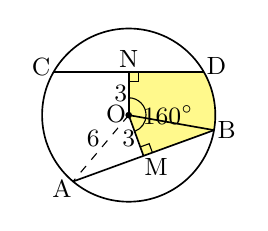
\begin{tikzpicture}[line width=0.6pt]
  \fill[yellow!45] (0.000,0.000) -- (0.000,0.550) -- (0.953,0.550) arc (29.990:-9.990:1.100) -- (0.188,-0.517) -- cycle;
  \draw (0.000,0.000) circle (1.100);
  \draw (-0.953,0.550) -- (0.953,0.550);
  \draw (-0.707,-0.843) -- (1.084,-0.191);
  \draw (0.000,0.000) -- (0.000,0.550);
  \draw (0.000,0.000) -- (0.188,-0.517);
  \draw (0.000,0.000) -- (1.084,-0.191);
  \draw[dashed, line width=0.4pt] (0.000,0.000) -- (-0.707,-0.843);
  \fill (0.000,0.000) circle (1.2pt);
  \draw[line width=0.4pt] (0.120,0.550) -- (0.120,0.430) -- (0.000,0.430);
  \draw[line width=0.4pt] (0.301,-0.476) -- (0.260,-0.363) -- (0.147,-0.404);
  \draw[line width=0.4pt] (0.000,0.220) arc (90.000:-70.000:0.220);
  \node[font=\small, inner sep=1.5pt] at (0.500,0.000) {$160^\circ$};
  \node[font=\small, inner sep=1.5pt] at (-0.100,0.280) {$3$};
  \node[font=\small, inner sep=1.5pt] at (0.000,-0.300) {$3$};
  \node[font=\small, inner sep=1.5pt] at (-0.450,-0.300) {$6$};
  \node[font=\small, inner sep=1.5pt] at (-0.160,0.020) {O};
  \node[font=\small, inner sep=1.5pt] at (0.000,0.710) {N};
  \node[font=\small, inner sep=1.5pt] at (-1.113,0.610) {C};
  \node[font=\small, inner sep=1.5pt] at (1.113,0.630) {D};
  \node[font=\small, inner sep=1.5pt] at (-0.847,-0.943) {A};
  \node[font=\small, inner sep=1.5pt] at (1.244,-0.191) {B};
  \node[font=\small, inner sep=1.5pt] at (0.348,-0.657) {M};
\end{tikzpicture}
